\chapter{Réalisation du programme}
\section{Structures de données}
	
Certaines des structures de données ne sont utilisées que par certains modules du programme. Il n'est donc pas nécessaire de les abstraire. En revanche, certaines de ces structures sont utilisées par plusieurs modules, c'est le cas de la liste chaînée.
	\subsection{Structures simples}
    
	\subsubsection{La structure map}
    La structure map est construite par le parseur de cartes, contenu dans le module de parsing.
	les champs de cette structure sont :
	\begin{itemize}
		\item Un entier hauteur
		\item Un entier largeur
		\item Un tableau de caractères
		\item Une structure position pour repérer le point de départ
		\item Un entier pour le maximum de checkpoints
	\end{itemize}	
    
	\subsubsection{La structure steps}
	La structure steps est un ensemble de coups relatifs à une carte. Elle est générée par le parseur de coups. Elle peut être utilisée,par exemple, pour de comparer les performences d'autres intelligences artificelles.\\
Elle contient : 
	\begin{itemize}
		\item Un entier pour le nombre d'accélérations
		\item Un entier pour le nombre d'étapes
		\item Une structure point pour la position de départ
		\item Deux tableaux de structures point contenant les positions et vitesses correspondantes
	\end{itemize}	
	\subsubsection{La structure point}
    Cette structure est exclusivement utilisée par les modules de moteur de jeu, ainsi que l'affichage graphique. \\
	La structure point est une structure simple à deux champs entiers. Ces deux nombres représentent une position sur la grille. Le moteur de jeu utilise cette structure pour communiquer une position à l'interface.\\
	
	\subsubsection{La structure node}
    La structure node est utilisée par le module de résolution d'une carte. Elle contient quatre champs entiers, correspondants à une position et une vitesse. Elle contient de plus un champs pointeur sur le noeud précédent.\\

Grâce à l'abscence de typage des données dans la liste chaînée (pointeur void), nous pouvons stocker des données de n'importe quel type dans une liste chaînée, notemment les structures point (pour le moteur de jeu) et node (pour le solveur).



	\subsection{Structures abstraites}	
    La seule structure ayant été sujet d'une abstraction est la liste chaînée.
	\subsubsection{Mise en oeuvre}
	Le type de données utilisée içi est une liste doublement chainée	
	\begin{figure}[h]
	\centering
	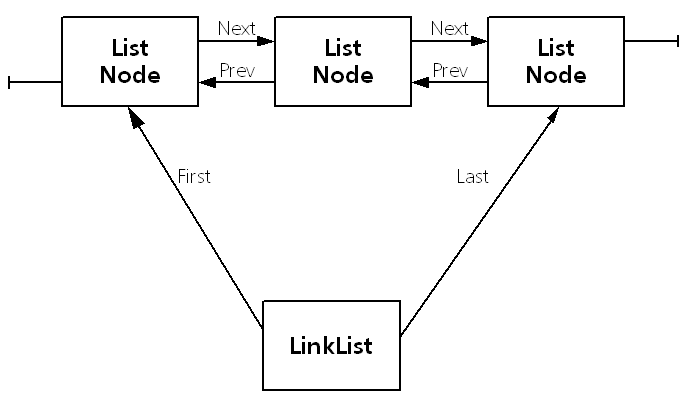
\includegraphics[scale = 0.3]{linklist.png}
    \caption{Double linked list}
    \end{figure} \\
    Les structures sont donc: \\
	\texttt{liste}
	\begin{itemize}
	\item pointeur sur l'élément tête
	\item pointeur sur l'élément queue
	\item entier nombre d'éléments (à 0 initialement)
	\end{itemize}
	\texttt{element}
    \begin{itemize}
	\item pointeur sans type sur une donnée
	\item pointeur élément sur l'élément précédent
	\item pointeur élément sur l'élément suivant
	\end{itemize}
	\subsubsection{Primitives}
  	Les primitives utilisées pour gérer la liste sont les suivantes : \\
	\texttt{list\_empty} qui teste si la liste est vide. \\
    \texttt{list\_head} renvoie la tête de la liste.\\
	\texttt{list\_tail} renvoie la queue de la liste. \\
    Celles relatives aux éléments sont :
	\texttt{list\_data} qui renvoie un pointeur sans type sur le champ donné de l'élément passé en paramètre.\\	
	\texttt{list\_next} renvoie le pointeur sur l'élément suivant. \\
	\texttt{list\_previous} renvoie le pointeur sur l'élément précédent. \\

	\subsubsection{Intérêt}
	L'abstraction de la liste chainée et de ses élements la rend utilisable par n'importe module sans qu'il n'ai connaissance de son implémentation. Cela permet notemmment de l'utiliser pour lister des coups jouables avec le solveur, ou de générer une liste de positions jouées. \\

	Le double chaînage permet de réduire la complexité de la fonction \texttt{list\_add} (qui effectue un ajout en queue). Avec une liste simple elle aurait été $\theta(n)$ en la taille de la liste, içi elle est en $\theta(1)$. De même pour la fonction de retrait en queue.\\








































\section{Le module SDL}

Un jeu pour qu'il en soit un a besoin d'une interface. Cette interface est indispensable pour le joueur. Sans elle il n'y aurait pas d'échange d'information entre l'utilisateur et la machine.

Nous avons fait le choix d'utiliser la bibliothèque SDL pour réaliser l'interface de vector racer. L'avantage de cette bibliothèque est qu'elle permet à la fois une gestion de l'affichage,du temps et des évènements (principalement les choix de l'utilisateur). Nous avions de plus  de l'expérience avec cette bibliothèque, ce qui a facilité notre choix.

Lien pour la bibliothèque SDL: http://www.libsdl.org

Les fonctions utilisant directement la SDL sont regroupées dans le module vectorSDL. A l'exception du module vectorGame, aucun autre module ne touche directement aux fonctions de la bibliothèque SDL. Nous avons fait ce choix afin de simplifier son utilisation.

\section{Moteur de jeu}

Le joueur va parcourir le circuit et traverser les différentes zones. Les évènements (les choix de l'utilisateur) sont traités grâce à des fonctions de la bibliothèque SDL.
Pour déterminer si le joueur perd,gagne ou triche, il faut que l'on vérifie à chaque étape la situation du joueur.

La première situation à vérifier est la colision avec un mur. On vérifie donc que le joueur ne tombe pas sur une case mur.
Nous n'avons pas traité le fait qu'un tracé peut traverser un mur sans s'y arrêter.

La deuxième situation est la fin du circuit. Pour gérer l'évènement, on considère le circuit comme terminé si le joueur est bien passé par toute les zones de checkpoint et qu'il est revenu soit sur la case départ, soit sur un checkpoint inférieur en valeur aux deux dernier checkpoint.

Enfin, il faut vérifier que le joueur ne rate pas un checkpoint. Pour cela on crée un compteur qui vérifie que la valeur du dernier checkpoint atteint augmente bien de manière régulière (sans sauts). 

\section{Mise en oeuvre de l'algorithme de résolution}
\subsection{Implémentation}
Nous avons implémenté l'algorithme de recherche en largeur en utilisant une structure noeud (cf. FIgure~\ref{noeud}). Cette structure contient 4 entiers représentant la position dans la grille et la vitesse en cette position. De plus elle contient un pointeur sur un noeud qui va servir à retracer le chemin qui a généré ce noeud.

\begin{figure}[h]
\centering
\begin{minipage}[c]{0.5\linewidth}
\begin{verbatim}
Struct node{
int x,y,dx,dy;
struct node * parent;
}
\end{verbatim}
\end{minipage}
\caption{Définition de struct noeud}
\label{noeud}
\end{figure}
Pour stocker ces noeud nous utilisons une structure liste. L'algorithme manipule deux listes pricipales : "queue" et "colored" en plus d'une liste temporaire "successors". La liste "queue" sert à stocker les noeuds 'candidats' qui potentiellement font avancer le chemin le plus vers la destination. "colored" quand à elle sert à mémoriser les noeuds déjà essayés. "successors" est une liste qui stocke temporairement tous les successeurs de la position courante.

Au début de l'algorithme, la liste "queue" contient uniquement la position de départ correspondant à une '*' dans la grille. Une fonction "generate-successors" s'occupe de générer les noeuds successeurs de cette position, il y'en a au maximum neuf, correspondant aux neuf accélérations possibles. Ces noeud successeurs sont générés dans l'ordre faisant maximiser la norme de la vitesse. Dans ce sens où le noeud de norme la plus grande est généré à la fin. Ensuite les champs parents de ces successeurs pointeront sur le noeud qui les a générés (le noeud source). Pour chacun de ces successeurs, l'algorithme va tester si sa position corrspond à une position destination. Si ce n'est pas le cas et qu'il n'a pas déjà été visité, il sera ajouté à "queue". L'étape suivante consiste à rajouter le noeud source à "colored" et continuer la recherche à partir du dernier élément de "queue". Ce processus sera répété jusqu'à ce que l'algorithme tombe sur un noeud destination et que le chemin parcouru soit valide, ou alors la liste "queue" devienne vide. 

Pour décider de la validité du chemin parcouru, une fonction "valid-path" a été implémenté. Elle retrace les neouds parcourues grâce au champs parent, et vérifie que le chemin passe par toutes les zones dans l'ordre croissant. Elle vérifie aussi si toutes les positions sont valides dans la grille. Par contre elle ne vérifie pas le fait que l'on puisse sauter sur des obstacles.

D'autres fonctions auxiliaires, mais très importantes, ont été impléméntés. Notamment "identify-zones" qui identifie les zones d'une map et "order-of-accelerations" qui ordonne les accélérations selon la norme.
\subsection{Tests et performances}

Nous avons testé notre algorithme sur plusieurs grilles de tailles différentes. La Figure~\ref{solution} montre un exemple de résolution sur une carte de taille 30x30. La liaison avec le module SDL permet de visualiser la validité de la solution proposée par l'algorithme, cependant nous ne disposons d'aucune outil permettant de confirmer l'optimisation.

Généralement, notre solveur propose des solutions instantanée pour des grilles d'ordre inférieur à 100x100. Il faut présiser que notre solver ne vérifie pas si une grille est valide avant de la résoudre.

Nous avons aussi envisgé de tester toutes les parties de notre algorithme. Ou à la limite ses fonctions pricipales. Mais la réalisations de ses tests s'est avérée insuffisante pour en tier des conclusions, puisque nous nous sommes basés sur des cas très particuliers qui ne peuvent être généralisés.
\begin{figure}[h]
\centering 
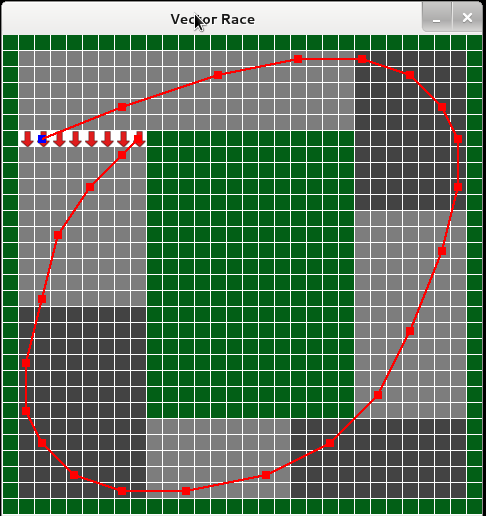
\includegraphics[scale=0.5]{Capture_du_2014-05-27_22-22-04.png}
\caption{Exemple de résolution}\label{solution}
\end{figure}